\documentclass[a4paper,14pt]{extarticle}

\usepackage[utf8x]{inputenc}
\usepackage[T1,T2A]{fontenc}
\usepackage[russian]{babel}
\usepackage{hyperref}
\usepackage{indentfirst}
\usepackage{here}
\usepackage{array}
\usepackage{graphicx}
\usepackage{caption}
\usepackage{subcaption}
\usepackage{chngcntr}
\usepackage{amsmath}
\usepackage{amssymb}
\usepackage{pgfplots}
\usepackage{pgfplotstable}
\usepackage[left=2cm,right=2cm,top=2cm,bottom=2cm,bindingoffset=0cm]{geometry}
\usepackage{multicol}
\usepackage{askmaps}
\usepackage{titlesec}
\usepackage{listings}
\usepackage{color}
\usepackage{courier}

\definecolor{green}{rgb}{0,0.6,0}
\definecolor{gray}{rgb}{0.5,0.5,0.5}
\definecolor{purple}{rgb}{0.58,0,0.82}

\lstset{
	language=Verilog,
	backgroundcolor=\color{white},   
	basicstyle=\small\ttfamily,
	commentstyle=\color{green},
	keywordstyle=\color{blue},	
	numberstyle=\tiny\color{gray},
	stringstyle=\color{purple},
	breakatwhitespace=false,
	breaklines=true,
	captionpos=b,
	keepspaces=true,
	numbers=left,
	numbersep=5pt,
	showspaces=false,
	showstringspaces=false,
	showtabs=false,
	tabsize=4,
	frame=single,
	inputpath={../quartus/},
	literate={~} {$\sim$}{1}
}

\renewcommand{\le}{\ensuremath{\leqslant}}
\renewcommand{\leq}{\ensuremath{\leqslant}}
\renewcommand{\ge}{\ensuremath{\geqslant}}
\renewcommand{\geq}{\ensuremath{\geqslant}}
\renewcommand{\epsilon}{\ensuremath{\varepsilon}}
\renewcommand{\phi}{\ensuremath{\varphi}}
\renewcommand{\thefigure}{\arabic{figure}} 	
\renewcommand*\not[1]{\overline{#1}}

\titleformat*{\section}{\large\bfseries} 
\titleformat*{\subsection}{\normalsize\bfseries} 
\titleformat*{\subsubsection}{\normalsize\bfseries} 
\titleformat*{\paragraph}{\normalsize\bfseries} 
\titleformat*{\subparagraph}{\normalsize\bfseries} 

\counterwithin{figure}{section}
\counterwithin{equation}{section}
\counterwithin{table}{section}
\newcommand{\sign}[1][5cm]{\makebox[#1]{\hrulefill}}
\graphicspath{{../pics/}}
\captionsetup{justification=centering,margin=1cm}
\def\arraystretch{1.3}
\setlength\parindent{5ex}
\titlelabel{\thetitle.\quad}

\begin{document}

\begin{titlepage}
\begin{center}
	Санкт-Петербургский Политехнический Университет Петра Великого\\[0.3cm]
	Институт компьютерных наук и технологий \\[0.3cm]
	Кафедра компьютерных систем и программных технологий\\[4cm]
	
	\textbf{ОТЧЕТ}\\ 
	\textbf{по лабораторной работе}\\[0.5cm]
	\textbf{SystemVerilog №4}\\[0.1cm]
	Автоматизация проектирования\\ дискретных устройств\\[4.0cm]
\end{center}

\begin{flushright}
	\begin{minipage}{0.45\textwidth}
		\textbf{Работу выполнил студент}\\[3mm]
		группа 33501/4 \hspace*{9mm} Дьячков В.В.\\[5mm]
		\textbf{Преподаватель}\\[5mm]
		\sign[1.5cm] \hspace*{1mm} к.т.н., доц. Филиппов А.С. \\[5mm]
	\end{minipage}
\end{flushright}

\vfill

\begin{center}
	Санкт-Петербург\\
	\the\year
\end{center}
\end{titlepage}

\addtocounter{page}{1}
\counterwithin{lstlisting}{section}

\tableofcontents
%\listoffigures
\newpage

\section{Цель работы}

\begin{itemize}
	\item Создать и исследовать генератор сигналов сложной формы на основе блока памяти ROM;
	\item Получение навыков работы с ISMCE (In-System Memory Content Editor).
\end{itemize}

\section{Ход работы}

\subsection{Создание и ввод проекта}

Создадим Verilog-описание генератора, схема которого приведена на рис. \ref{fig:source}. Генератор содержит счетчик, который используется для последовательной адресации ROM. В памяти хранятся данные, интерпретируемые как периодический сигнал.
\begin{figure}[H]
	\centering
	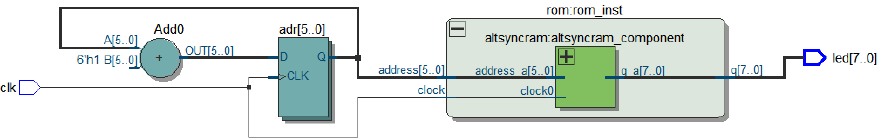
\includegraphics[width=\textwidth]{source}
	\caption{Схема генератора}
	\label{fig:source}
\end{figure}

\noindent На рис. \ref{fig:mif} приведен созданный инициализирующий файл \code{.mif} для ROM. 
\begin{figure}[H]
	\centering
	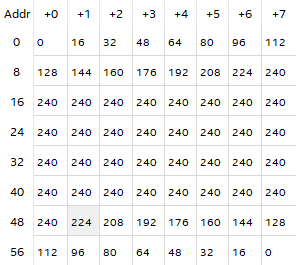
\includegraphics[scale=1]{mif}
	\caption{Инициализирующие значения ROM}
	\label{fig:mif}
\end{figure}

На основе мегафукцнии <<ROM: 1-PORT>> создадим модуль ROM, после чего создадим описание генератора. В листинге \ref{code:lab_ismce} приведен код программы на языке Verilog.

\lstinputlisting[caption=lab\_ismce.v, label=code:lab_ismce]{lab_ismce.v}

На рис. \ref{fig:rtl} изображена схема устройства в RTL Viewer, полученная после компиляции созданного проекта.
\begin{figure}[H]
	\centering
	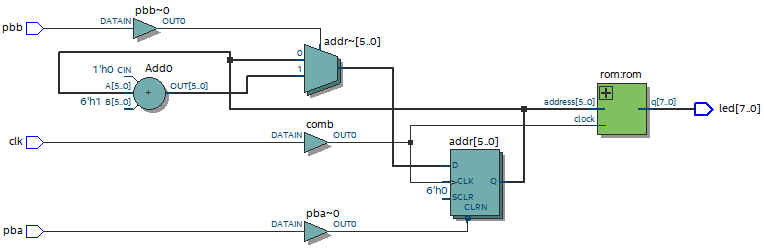
\includegraphics[width=\textwidth]{rtl}
	\caption{Схема устройства в RTL Viewer}
	\label{fig:rtl}
\end{figure}

\subsection{Создание экземпляра логического анализатора SignalTapII}

\begin{figure}[H]
	\centering
	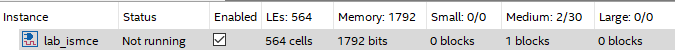
\includegraphics[width=\textwidth]{stp1}
	\caption{Схема устройства в RTL Viewer}
	\label{fig:rtl}
\end{figure}

\begin{figure}[H]
	\centering
	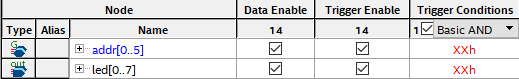
\includegraphics[scale=1]{stp2}
	\caption{Схема устройства в RTL Viewer}
	\label{fig:rtl}
\end{figure}

\subsection{Настройка и запуск ISMCE}

\subsection{Генерация заданного сигнала}

\section{Выводы}

\end{document}